% Created 2016-08-17 Wed 14:38
\documentclass[tikz]{standalone}

\usepackage[utf8]{inputenc}
\usepackage[T1]{fontenc}
\usepackage{helvet}
\usepackage{../../templates/msc}

\renewcommand{\familydefault}{\sfdefault}

\tikzset{
every picture/.style={
line width=1pt
}}

\usepackage{tikz}
\author{Holger Karl}
\date{\today}
\title{}




\usetikzlibrary{graphs}

\begin{document}
\begin{tikzpicture}
% 

 

% Servers: 
\node [draw, fill=blue!10] (s1)  {Server};
\foreach \i  [evaluate=\i as \previousi using \i-1] in {2,...,6} {
  \node [draw, fill=blue!10, right=of s\previousi] (s\i)  {Server};
}
\node [fill=red!10, draw, below= 0cm of s3] (l) {Leader};
\coordinate (tmp) at (1,1.5);
\node at (0,1.5) (zs) {Zookeeper Service};


\begin{pgfonlayer}{background}
  \node [rounded corners, draw, fill=green!5, fit=(s1) (s6) (l) (zs) ]
  {};
\end{pgfonlayer}
\foreach \i in {1,...,2} {
  \draw [->] (s\i.north) to[out=30] (s3.north);
}
\foreach \i in {4,...,6} {
  \draw [->] (s\i.north) to[out=150, in=30] (s3.north);
}

\node [below left=of s1,  draw, fill=yellow!10] (c1)  {Client};
\foreach \i  [evaluate=\i as \previousi using \i-1] in {2,...,8} {
  \node [draw, fill=yellow!10, right=of c\previousi] (c\i)  {Client};
}

\draw [->] (c1) -- (s1); 
\draw [->] (c2) -- (s1); 
\draw [->] (c3) -- (s2); 
\draw [->] (c4) -- (s2); 
\draw [->] (c5) -- (s2); 
\draw [->] (c6) -- (s4); 
\draw [->] (c7) -- (s4); 
\draw [->] (c8) -- (s6); 

\end{tikzpicture}


%--------------------- 
% 2: namespace 

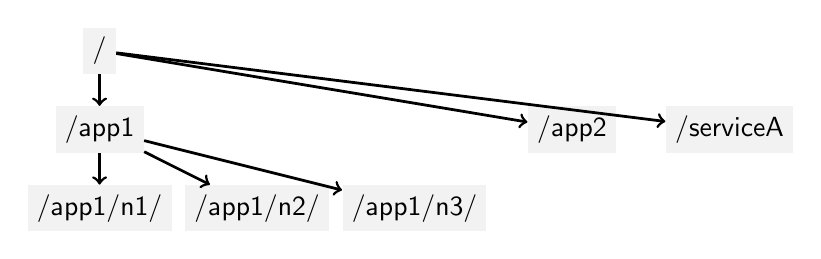
\begin{tikzpicture}
% \graph { \texttt{t} -> {b, c} -> d };
\graph [grow down, branch right=2cm, nodes={thin, fill=gray!10}] { "/" -> 
  {
    "/app1"  -> {
      "/app1/n1/", 
      "/app1/n2/", 
      "/app1/n3/"
    },
    "/app2", 
    "/serviceA"
  }  };
\end{tikzpicture}


\end{document}